\section{Einführung ``Mikrobenparade''}
\begin{enumerate}
	\item Welches sind die Merkmale des Lebens? Warum sind Prionen keine Lebewesen? Warum können sie trotzdem infektiös sein? \hfill \vspace{4mm}

	Merkmale des Lebens sind zum Beispiel ein Stoffwechsel, Fortpflanzung \& Evolution.
	Prionen haben keinen eigenen Stoffwechsel und keine Erbinformationen (DNA, RNA)
	die ``chemischen'' Fähigkeiten der Proteine reichen für das Übernehmen von fremden Zellen aus.
	%Durch die Übernahme der Zellen sind sie mit ihrem eigenen Erbgut in der Lage,
	%sich zu vermehren - deshallb sind sie infektiös.
	



	\item Nennen Sie mindestens fünf durch Bakterien verursachte Krankheitserreger, die Namen der entsprechenden Bakterien sowie die Bakteriengruppen, denen sie zuzuordnen sind!
		\label{item:boesebakterien}
	\begin{enumerate}[label=\arabic*)]
		\item \emph{Yersinia pestis} \hfill \\
			Pest, Gammaproteobacteria
		\item \emph{Vibrio cholerae} \hfill \\
			Cholera, Proteobacteria
		\item \emph{Bordetella pertussis} \hfill \\
			Keuchhusten, Proteobacteria
		\item \emph{Mycoplasma pneumoniae} \hfill \\
			Lungenentzündung, Firmicutes
		\item \emph{Bacillus anthracis} \hfill \\
			Milzbrand, Clostridien
	\end{enumerate}


	\item Welche Rolle spielen die Plasmide für die Virulenz von \emph{Bacillus anthracis}?  \hfill \vspace{0.2mm} \\

		Die Virulenz von \emph{Bacillus anthracis} ergibt sich
		aus den Plasmiden ``px01'' und ``px02''.
		Im ersten Plasmid (``px01'') wir ein potentes Toxin codiert,
		das zweite Plasmid (``px02'') ist für die Bildung einer Kapsel verantwortlich.
		Durch die Kapsel wird die Phagocytose der Zelle verhindert,
		wodurch das Toxin wirken kann.


	\item Nennen Sie einige Bakterien, die für die Landwirtschaft/unsere Ernährung von entscheidender Bedeutung sind. \hfill \\
	
	\emph{Saccharomyces cerevisae}, die Bier- \& Bäckerhefe,
	ist ein wichtiger Teil der Nahrungsmittelproduktion.
	\emph{Lactobacillus casei} ermöglicht die zum Beispiel die Herstellung von Sauerkraut,
	und das Haltbarmachen von Milchprodukten.
	Diverse Arten von \emph{Rhizobium} ermögliche die Fixierung von molekularen Stickstoff,
	den sie den Wurzeln von Pflanzen bereitstellen.
	Diese, sogenannten ``Knölchenbakterien'', sind Grundlesgen für die Stickstoffversorgung der Pflanzen.
\end{enumerate}

\section{Geschichte der Mikrobiologie}
\begin{enumerate}
	\item Womit beschäftigen sich die Koch’schen Postulate?
	Bei welcher Gelegenheit wurden Sie von Robert Koch aufgestellt und was besagen sie? \hfill \vspace{4mm}

	\begin{enumerate}[label=\arabic*)]
		\item In einem Infizierten Organismus müssen Erreger nachweisbar sein.
		\item Die offenbaren Errger müssen in reiner form isoliert werden.
		\item Mit den Reinkulturen müssen gesunde Organismen identifiuert werden können.
	\end{enumerate}
	Sie wurden von Robert Koch während der Entdeckung von \emph{Bacillus anthracis},
	dem Erreger des Milzbrandes aufgestellt,
	um zu Ermitteln ob die Bakterien Folge oder Ursache der Krankheit sind.	
	

	\item In einem klassischen Experiment konnte Griffith 1928 einen apathogenen Stamm von
	\emph{Streptococcus pneumoniae} in einen pathogenen Stamm umwandeln.\\
	Wie funktionierte dieses Experiment? Worauf beruht es? 
	Welche bahnbrechende Schlußfolgerung wurde daraus gezogen? \hfill \vspace{4mm}
	
	\begin{figure}[ht!]
	\leavevmode
	\begin{center}
	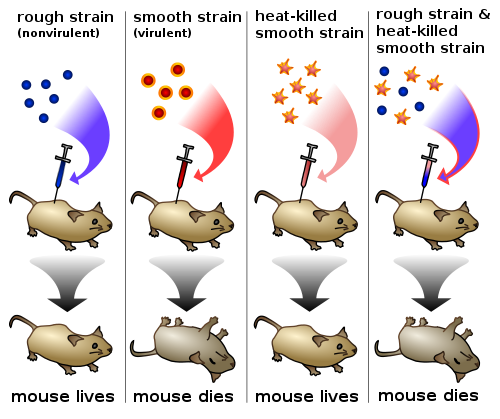
\includegraphics[scale=0.47]{./pictures/griffith_exp_500}
	\end{center}
	\caption{\slshape{Griffith's Experiment.}}
	\label{fig:griffith}
	\end{figure}

	Es gibt zwei Zelltypen von \emph{Streptococcus pneumoniae} der ``s''-Typ
	bildet eine Kapsel aus, und erscheint deshalb im Lichtmikroskop glatt (``smooth').
	Der \& ``r''-Typ, kann keine Kapsel ausbilden und erscheint im lichtmikroskopischen Bild
	mit einer rauen (``rough'') Oberflächen.
	Nur Zellen des ``s''-Typs lösen in Mäusen Lungenentzündung aus,
	die Zellen des ``r''-Typs sind sind nicht durch eine Kapsel geschützt und können
	vom Immunsystem erkannt und bekämpft werden.

	Grifith tötet, in dem nach ihm benannten Experiment,
	Bakterien des ``s''-Typs durch erhitzen ab.
	Werden einer Maus nur abgetötete Erreger des ``s''-Typs injeziert,
	bleibt dieses gesund.
	Werden sowohl abgetöte Bakterien des ``s''-Typs,
	als auch lebenden Bakterien des ``r''-Typs injeziert,
	erkrankt die Maus an einer Lungenentzündung.
	In der Maus befinden sich dann Zellen vom \emph{Streptococcus pneumoniae} 
	die eine Kapsel ausbilden.

	Griffith hat gezeigt, dass die Fähigkeit zur Kapselbildung von den toten ``s''-Zellen
	auf die lebenden ``r-''Zellen übertragen worden war.
	1944 wurde von Oswald Avery gezeigt,
	dass diese Transformation auf einer Übertragung von DNS beruhte.


	\item Mycoplasmen sind die wichtigsten Objekte der synthetischen Biologie. 
	Nennen Sie einige Eigenschaften dieser Bakterien,
	die sie für die Forschung allgemein und die synthetische Biologie im besonderen interessant machen. \hfill \vspace{4mm}

	Da die Mycoplasmen eines der kleinsten Genome besitzen sind sie besonderst für die synthetische Biologie interessant.
	Das Genom von \emph{Mycoplasma pneumoniae},
	dem Errreger der Pneumonie,
	umfasst beispielsweise nur 816 kBp mit 688 Genen.
	Regulation findet kaum statt.
	Bei \emph{Mycoplasma pneumoniae} handelt es sich um ein gram-positives Bakterium ohne Zellwand.
	Es haftet an, und bweget sich dann gleitend fort.
	Auch die nahe Verwandten von \emph{Mycoplasma pneumoniae},
	haben kleine Genome und sind meist pathogen.
	Das kleinste bekannte Genom hat \emph{Mycoplasma genitalium} mit 600 kBp.

	An ihnen lässt sich gut erkennen,
	welche Stoffwechsel funktionen für ``Leben'' obligat sind.
	Ein minimales Gen-Set lässt sich ermitteln und künstlich erzeugen.

\end{enumerate}
